\documentclass[tikz]{standalone}

\usepackage{fontspec}
\usepackage{unicode-math}
\usetikzlibrary{arrows.meta,positioning,shapes}
\setmainfont{TeX Gyre Pagella}
\setmathfont{TeX Gyre Pagella Math}
\setsansfont[Scale=0.95]{Clear Sans}
\setmonofont[
  Scale=1.05,
  UprightFeatures={SmallCapsFont=LMMonoCaps10-Regular},
  ItalicFeatures={SmallCapsFont=LMMonoCaps10-Oblique},
]{Latin Modern Mono}
% Patch for modern versions of fontspec:
\let\ttfamilyinline\relax
\newfontfamily\ttfamilyinline{Latin Modern Mono Prop}
% Adjust tikz settings:
\tikzset{
  > = {Stealth[length=2.8pt .8, inset'=0pt .575, width'=0pt 1.55, line join=round, sep]},
  normal linewidth/.style = semithick,
}



\begin{document}
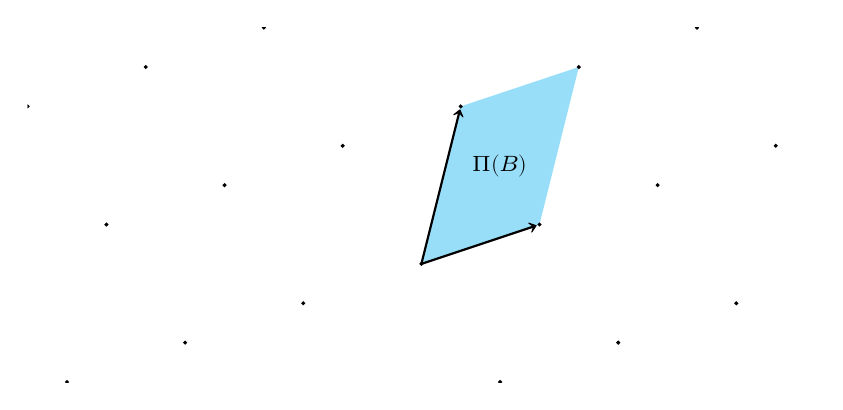
\begin{tikzpicture}[scale=0.5]
  \clip (-10, -3) rectangle (10, 6);
  \fill[color=cyan!40]
    (0, 0) -- (3, 1) -- ++(1, 4) -- (1, 4);
  \draw[->, thick] (0, 0) -- (3, 1);
  \draw[->, thick] (0, 0) -- (1, 4);
  \node at (2.0, 2.5) {\footnotesize$\Pi(B)$};

  \foreach \x in {-10,...,10}
  \foreach \y in {-10,...,10}
    \draw[fill] (3*\x + \y, \x + 4*\y) circle (1pt);
\end{tikzpicture}
\end{document}
